\documentclass[12pt,letterpaper]{article}

\newenvironment{proof}{\noindent{\bf Proof:}}{\qed\bigskip}

\newtheorem{theorem}{Theorem}
\newtheorem{corollary}{Corollary}
\newtheorem{lemma}{Lemma} 
\newtheorem{claim}{Claim}
\newtheorem{fact}{Fact}
\newtheorem{definition}{Definition}
\newtheorem{assumption}{Assumption}
\newtheorem{observation}{Observation}
\newtheorem{example}{Example}
\newcommand{\qed}{\rule{7pt}{7pt}}

\newcommand{\assignment}[4]{
\thispagestyle{plain} 
\newpage
\setcounter{page}{1}
\noindent
\begin{center}
\framebox{ \vbox{ \hbox to 6.28in
{\bf CS440: Introduction to Artificial Intelligence \hfill #1}
\vspace{4mm}
\hbox to 6.28in
{\hspace{2.5in}\large\mbox{In class assignment #2}}
\vspace{4mm}
\hbox to 6.28in
{{\it Handed Out: #3 \hfill Due: #4}}
}}
\end{center}
}

\newcommand{\solution}[4]{
\thispagestyle{plain} 
\newpage
\setcounter{page}{1}
\noindent
\begin{center}
\framebox{ \vbox{ \hbox to 6.28in
{\bf CS440 : Introduction to Artificial Intelligence \hfill #4}
\vspace{4mm}
\hbox to 6.28in
{\hspace{2.5in}\large\mbox{In class assignment #3}}
\vspace{4mm}
\hbox to 6.28in
{#1 \hfill {\it Handed In: #2}}
}}
\end{center}
\markright{#1}
}

\newenvironment{algorithm}
{\begin{center}
\begin{tabular}{|l|}
\hline
\begin{minipage}{1in}
\begin{tabbing}
\quad\=\qquad\=\qquad\=\qquad\=\qquad\=\qquad\=\qquad\=\kill}
{\end{tabbing}
\end{minipage} \\
\hline
\end{tabular}
\end{center}}

\def\Comment#1{\textsf{\textsl{$\langle\!\langle$#1\/$\rangle\!\rangle$}}}


\usepackage{algorithm}
\usepackage{listings}
%\usepackage{algpseudocode}
\usepackage{graphicx,amssymb,amsmath}
\usepackage{epstopdf}

\usepackage{pgf}
\usepackage{tikz}
\usetikzlibrary{arrows,automata}
\usepackage[latin1]{inputenc}

\sloppy


\oddsidemargin 0in
\evensidemargin 0in
\textwidth 6.5in
\topmargin -0.5in
\textheight 9.0in

\begin{document}

\solution{Dan McQuillan}{\today}{3}{Spring 2014}

\pagestyle{myheadings}  % Leave this command alone

\begin{enumerate}

	\item {\bf{Probability}}
	
		\begin{enumerate}
			
			\item{}
				Suppose:
				
				\[
					D = \left\{ 
						\begin{array}{ll}
							d_1 & \text{if disease affects you} \\
							d_2 & \text{if disease doesn't affect you} \\
						\end{array}
					 \right\}
				\]
				\[
					T = \left\{ 
						\begin{array}{ll}
							t_1 & \text{test was correct} \\
							t_2 & \text{test was a false positive} \\
						\end{array}
					 \right\}
				\]
				
				Then:
				
				\[
					P(D = d_1) = \frac{1}{8000}
				\]
				\[
					P(T | D) = 0.97
				\]
				\[
					P( \neg T | \neg D) = 0.97 \rightarrow P(T | \neg D) = 1 - P(\neg | \neg D) = 0.03
				\]
				\[
					P(D = d_1 | T = t_1) = \alpha \left< 0.97 (0.000125), (1 - 0.97)(1 - \frac{1}{8000} \right>
				\]
				\[
					P(D = d_1 | T = t_1) = \alpha \left< 0.00012125, 0.02999625 \right> \cdot \frac{1}{0.00012125 + 0.02999625}
				\]
				\[
					P(D = d_1 | T = t_1) = \alpha \left<0.00402589856395783, 0.995974101436042 \right>
				\]
				\[
					P(D = d_1 | T = t_1) = 0.00402589856395783
				\]
				
				No, you shouldn't have anything to worry about.
				
				
				
%				\[
%					P(D = d_1) = 0.000012
%				\]
				
%				\[
%					P(A = a_2) = 1 - P(A = a_1) = 0.9999875
%				\]
%				
%				\[
%					P(B = b_1) = 0.97
%				\]
%				\[
%					P(B = b_2) = 1 - P(B = b_1) = 0.03
%				\]
%				
%				Given that A and B are independent we know that:
%				\[
%					P(A \wedge B) = P(A)P(B)
%				\]
%				
%				Therefore:
%				\[
%					P(A = a_1 | B = b_1) = \frac{P(A = a_1 \wedge B = b_1)}{P(B = b_1)} = \frac{P(A = a_1)P(B = b_1)}{P(B = b_1)} = P(A = a_1)
%				\]
%				
%				The probability is very low of actually having the disease with a probability of:
%				\[
%					P(A = a_1 | B = b_1) = 0.000012
%				\]
%				And you probably should not be worried. \\
			\item{}
			
				Suppose:
				
				We have a random variable M:
				\[
					M = \left\{
						\begin{array}{ll}
							r & \text{ if the marble is red } \\
							b & \text{ if the marble is blue } \\
						\end{array}
					\right\}
				\]
				
				Given by the information we know that:
				\[
					P(M = r) = 0.30
				\]
				\[
					P(M = b) = 0.70
				\]
				
				We know that we have a uniform distribution since \( \Sigma_{m \in M} P(M = m) \le 1 \).
				
				Therefore:
				
				\[
					P(M = r \wedge M = r) = P(M = r) P(M = r) = (0.3)(0.3) = 0.09
				\]
				
				\[
					P(M = b \wedge M = b) = P(M = b) P(M = b) = (0.7)(0.7) = 0.49
				\]
					
				\[
					P(M = r \wedge M = b) = P(M = r) P(M = b) = (0.3)(0.7) = 0.21
				\]
					
				\[
					P(M = b \wedge M = r) = P(M = r) P(M = b) = (0.3)(0.7) = 0.21
				\]
				Suppose you select one of your two marbles at random.  What is the probability that it is blue? \\
				\[
					P(M = b | M = r \wedge M = b) = 0.21
				\]
				\[
					P(M = b | M = b \wedge M = b) = 0.49
				\]
				\[
					P(M = b) = 0.7
				\]
			
		\end{enumerate}
	
 	\item {\bf{Bayesian Networks}}
	
		Special Exhibits:
		
		\[
			E = \left\{
				\begin{array}{ll}
					g & \text{ if Gourmet Food } \\
					a & \text{ if art on loan } \\
					e & \text{ if empty } \\
				\end{array}
			\right\}
		\] \\
		
		Thieves:
		
		\[
			T = \left\{
				\begin{array}{ll}
					t & \text{ if will steal } \\
					f & \text{ if won't steal } \\
				\end{array}
			\right\}
		\] \\
		
		Weather:
		
		\[
			W = \left\{
				\begin{array}{ll}
					h & \text{ if hot } \\
					c & \text{ if cold } \\
					n & \text{ if neutral } \\
				\end{array}
			\right\}
		\] \\
		
		Alarm:
		
		\[
			A = \left\{
				\begin{array}{ll}
					t & \text{ if alarm sounded } \\
					f & \text{ if alarm didn't sound } \\
				\end{array}
			\right\}
		\] \\
		
		Rats:
		
		\[
			R = \left\{
				\begin{array}{ll}
					t & \text{ if rats } \\
					f & \text{ if no rats } \\
				\end{array}
			\right\}
		\] \\
		
		Insurance claim:
		
		\[
			I = \left\{
				\begin{array}{ll}
					t & \text{ if insurance claim } \\
					f & \text{ if no insurance claim } \\
				\end{array}
			\right\}
		\] \\
		
		Overtime:
		
		\[
			O = \left\{
				\begin{array}{ll}
					t & \text{ if overtime } \\
					f & \text{ if no overtime } \\
				\end{array}
			\right\}
		\] \\
	
	 \begin{enumerate}
		 \item{}
			\vspace*{4mm}
			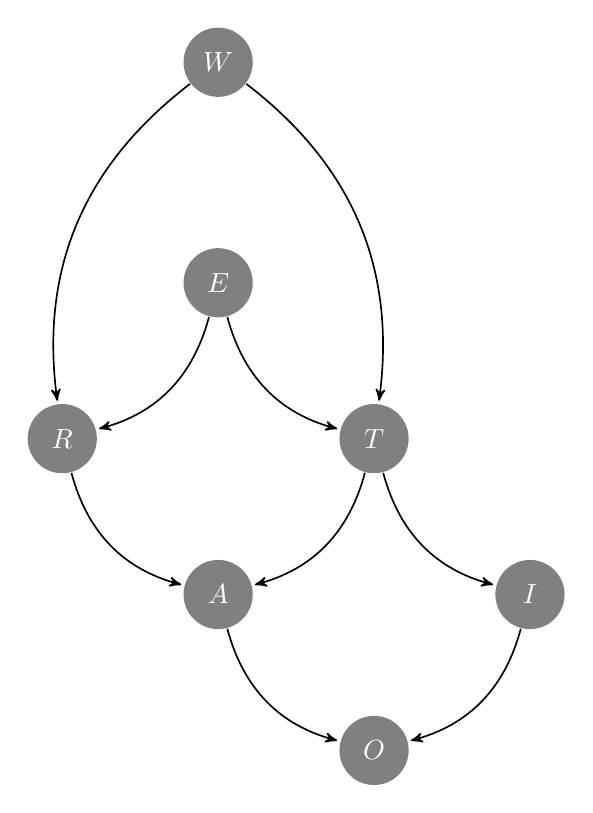
\begin{tikzpicture}[->,>=stealth',shorten >=1pt,auto,node distance=2.8cm,semithick]
				  \tikzstyle{every state}=[fill=gray,draw=none,text=white]
				
				  \node[state] 	     (W)                    {$W$};
				  \node[state]         (E) [below of=W] {$E$};
				  \node[state]         (R) [below left of=E] {$R$};
				  \node[state]         (T) [below right of=E] {$T$};
				  \node[state]         (A) [below right of=R]       {$A$};
				  \node[state]         (I) [below right of=T]       {$I$};
				  \node[state]         (O) [below right of=A]       {$O$};
				
				  \path
				  	(W) edge [bend right] node {} (R)
					       edge [bend left] node {} (T)
				  	(E) edge [bend left] node {} (R)
					       edge [bend right] node {} (T)
				  	(R) edge [bend right] node {} (A)
					(T) edge [bend left] node {} (A)
					(T) edge [bend right] node {} (I)
					(A) edge [bend right] node {} (O)
					(I) edge [bend left] node {} (O);
			\end{tikzpicture}
		
		\item{} This structure is a polytree since it is a directed, acyclic graph. This is because for every vertex there is no way to get back to vertex v.
		\item{} 287 parameters are needed for the full joint probability.
		\item{} Baye's net parameters: \\
	
			\(
				\begin{array}{l|l}
					W & P(W) \\
					\hline
					h & (a) \\
					c & (b) \\
					n & (c) \\
				\end{array}
			\)
			\(
				\begin{array}{l|l}
					E & P(E) \\
					\hline
					g & (d) \\
					a & (e) \\
					e & (f) \\
				\end{array}
			\)
			\(
				\begin{array}{ll|l}
					E & W & P(R|W,E) \\
					\hline
					g & h & (g) \\
					g & e & (h) \\
					g & n & (i) \\
					a & h & (j) \\
					a & e & (k) \\
					a & n & (l) \\
					e & h & (m) \\
					e & e & (n) \\
					e & n & (o) \\
				\end{array}
			\)
			\(
				\begin{array}{ll|l}
					E & W & P(T|W,E) \\
					\hline
					g & h & (p) \\
					g & e & (q) \\
					g & n & (r) \\
					a & h & (s) \\
					a & e & (t) \\
					a & n & (u) \\
					e & h & (v) \\
					e & e & (w) \\
					e & n & (x) \\
				\end{array}
			\) \\ \\
			
			\(
				\begin{array}{ll|l}
					R & T & P(A|R,T) \\
					\hline
					t & t & (y) \\
					t & f & (z) \\
					f & t & (aa) \\
					f & f & (ab) \\
				\end{array}
			\)
			\(
				\begin{array}{l|l}
					T & P(I|T) \\
					\hline
					t & (ac) \\
					f & (ad) \\
				\end{array}
			\)
			\(
				\begin{array}{ll|l}
					A & I & P(O|A,I) \\
					\hline
					t & t & (ae) \\
					t & f & (af) \\
					f & t & (ag) \\
					f & f & (ah) \\
				\end{array}
			\) \\ \\
			34 parameters required for the baye's net \\
			Savings \( \rightarrow \) 287 - 34 = 253 less parameters. \\
		
		\item{} Find the markov blankets for each of the 7 variables:
		
			MB(W) = \{ R, T, E \} \\
			MB(E) = \{ R, T, W \} \\
			MB(R) = \{ W, E, A, T \} \\
			MB(T) = \{ W, E, A, I, R \} \\
			MB(A) = \{ R, T, O, I \} \\
			MB(I) = \{ T, O, A \} \\
			MB(O) = \{ A, I \} \\
			
		\item{}
		
			No, the alarm going off is not conditionally independent of the insurance claim being submitted, given that there are rats. \\
			
			This is a result of the random variable, R, having no influence on the random variable, I. The only influencing variable for I is whether or not the thieves did damage. \\
			
	\end{enumerate}
	
	\item {\bf{Probabilities in Bayesian Networks}}
	
	\begin{enumerate}
		\item{}
			\(
				P(A) = 0.00972 + 0.00972 + 0.00054 + 0.00144 + 0.08748 + 0.00648 + 0.00486 + 0.00096 + 0.01458 + 0.00648 + 0.00216 + 0.00036 + 0.13122 + 0.00432 + 0.01944 + 0.00024
			\) \\
			\(
				P(A) = 0.3
			\) \\ \\ 
			
			\(
				P( \neg A) = 0.01008 + 0.13608 + 0.00056 + 0.2016 + 0.09072 + 0.09072 + 0.00504 + 0.01344 + 0.01512 + 0.09072 + 0.00224 + 0.00504 + 0.13608 + 0.06048 + 0.02016 + 0.00336
			\) \\
			\(
				p( \neg A) = 0.7
			\) \\ \\
			
			\(
				P(B) = 0.00972 + 0.00972 + 0.08748 + 0.00648 + 0.01458 + 0.00648 + 0.13122 + 0.00432 + 0.01008 + 0.13608 + 0.09072 + 0.09072 + 0.01512 + 0.09072 + 0.13608 + 0.06048
			\) \\
			\(
				P(B) = 0.9
			\) \\ \\
			
			\(
				P(C|A) = 0.00972 + 0.08748 + 0.01458 + 0.13122 + 0.00054 + 0.00486 + 0.00216 + 0.1944
			\) \\
			\(
				P(C|A) = 0.27
			\) \\ \\
			
			\(
				P(C| \neg A) = 0.01008 + 0.09072 + 0.01512 + 0.13608 + 0.00056 + 0.00504 + 0.00224 + 0.02016
			\) \\
			\(
				P(C| \neg A) = 0.28
			\) \\ \\
			
			\(
				P(D|B,C) = 0.00972 + 0.08748 + 0.01008 + 0.09072
			\) \\
			\(
				P(D|B,C) = 0.198
			\) \\ \\
			
			\(
				P(D|B,\neg C) = 0.00972 + 0.00648 + 0.13608 + 0.09072
			\) \\
			\(
				P(D|B,\neg C) = 0.243
			\) \\ \\
			
			\(
				P(D| \neg B, C) = 0.00054 + 0.00486 + 0.00056 + 0.00504
			\) \\
			\(
				P(D| \neg B, C) = 0.011
			\) \\ \\
			
			\(
				P(D| \neg B, \neg C) = 0.00144 + 0.00096 + 0.02016 + 0.01344
			\) \\
			\(
				P(D| \neg B, \neg C) = 0.036
			\) \\ \\
			
			\(
				p(E|C) = 0.00972 + 0.00054 + 0.01008 + 0.00056 + 0.01458 + 0.00216 + 0.01512 + 0.00224
			\) \\
			\(
				P(E|C) = 0.055
			\) \\ \\
			
			\(
				P(E|\neg C) = 0.00972 + 0.00144 + 0.13608 + 0.02016 + 0.00648 + 0.00036 +0.09072 + 0.00504
			\) \\ 
			\(
				P(E|\neg C) = 0.27
			\) \\ 
		
		\item{} Express�P(D�|�B)�using�the�probabilities�you�calculated \\
		
			\(
				\begin{array}{ll}
					P(D|B) & = \Sigma_{a \in A} \Sigma_{c \in C} P(A,B,C,D) =  \Sigma_{a \in A} \Sigma_{c \in C} P(A)P(B)P(C|A)P(D|B,C) \\ \\
						   & = P(B) \Sigma_{a \in A} p(A)  \Sigma_{c \in C} P(C|A)P(D|B,C) \\ \\
					P(D|B) & = P(B) \{ P(a) \left[ P(c|a)P(D|B,c) + P(\neg c | a) P(D|B, \neg c) \right] \\
						   & \hspace{8mm} + P(\neg a) \left[ P(c|\neg a) P(D|B,c) + P(\neg c|\neg a)P(D|B,\neg c) \right] \} \\
				\end{array}
			\)

		\item{} Use�the�calculated�values�from�part�(a)�to�obtain�the�value�of�P(D�|�B). \\
		
			\(
				\begin{array}{ll}
					P(D|B) & = (0.9) \{ (0.3) [ (0.27)(0.198) + (0.03)(0.243)] + (0.7)[(0.28)(0.198) + (0.42)(0.243)]\} \\ \\
						   & = (0.9) [(0.3)(0.06075) + (0.7)(0.1575)] \\ \\
					P(D|B) & = 0.1156275 
				\end{array}
			\) \\
		
		\item{} Compute�the�following�probabilities
		
			\begin{enumerate}
				\item{} \( P(E | A) \) \\
					
					\(
						\begin{array}{ll}
							P(E | A) & = \alpha \Sigma_{c \in C} P(A,E,C) = \alpha \Sigma_{c \in C} P(E | C) P(C | A) P(A) \\ \\
								     & = \alpha P(A) \Sigma_{c \in C} (P(E | C) P(C | A) \\ \\
								     & = P(A) [ P(E | c) P(c | A) + P(E | \neg c)P(\neg c | A) ] \\ \\
							P(E | A) & = 0.006885 \\ \\
						\end{array}
					\)					
					
				\item{} \( P(A | B) \) \\
					
					\(
						P(A | B) = \frac{P(B | A) P(A)}{P(B)}
					\) \\ \\
					
					\(
						\begin{array}{ll}
							P(D | B) & = \Sigma_{a \in A} \Sigma_{c \in C} P(A,B,C,D) \\ \\
								      & = \Sigma_{a \in A} \Sigma_{c \in C} P(A)P(B)P(C | A)P(D | B,C) \\ \\
								      & = P(A)P(B) \Sigma_{c \in C} \Sigma_{d \in D} P(C | A)P(D | B,C) \\ \\
								      & = P(A)P(B) [ P(c | A) P(d | B, c) + P(c | A) P(\neg d | B, c) \\
								      & \hspace{4mm} +P(\neg c | A) P(d | B, \neg c) + P(\neg c | A) P(\neg d | B, \neg c) ] \\ \\
								      & = (0.3)(0.9) [ (0.27)(0.198) + (0.27)(0.43308) + (0.03)(0.243) + (0.03)(0.162)] \\ \\
								      & = (0.3)(0.9)(0.1825416) \\ \\
							P(D | B)  & = 0.049286232 \\ \\
						\end{array}
					\)					

				\item{} \( P(B,D | C) \) \\
				
					\(
						P(B,D | C) = \frac{ P(C | B,D)P(B,D) }{ P(C) } = \frac{ P(C | B,D)P(B)P(D | B)}{P(C)}
					\) \\ \\
					
					\(
						\begin{array}{ll}
							P(C) & = \alpha \Sigma_{a \in A} P(A,C) \\ \\
								& = \alpha \Sigma_{a \in A} P(A) P(C | A) \\ \\
								& = P(a) P(C | a) + P( \neg a ) P(C | \neg a) \\ \\
								& = (0.3)(0.27) + (0.7)(0.28) \\ \\
								& = 0.277 \\ \\
						\end{array}
					\)
					
					\(
						\hspace{1mm}P(D | B) = 0.441
					\) \\ 
					
					\(
						\begin{array}{ll}
							P(C | D,B) & = \Sigma_{a \in A} \Sigma_{c \in C} P(A,B,C,D) \\ \\
									& = \Sigma_{a \in A} P(A) P(B) P(C | A) P(D | B,C) \\ \\
									& = P(B) P(D | B,C) \Sigma_{a \in A} P(A) P(C | A) \\ \\
									& = P(B) P(D | B, C) [ P(a) P(C | a) + P( \neg a) P(C | \neg a) \\ \\
									& = P(B)P(D | B,C)P(C) \\ \\
							P(C | D,B) & = (0.9)(0.198)(0.277) = 0.0493614 \\ \\
						\end{array}
					\) \\
										
					\(
						P(B,D | C) = \frac{ P(C | B,D)P(B)P(D | B)}{P(C)} = \frac{ (0.0493614)(0.9)(0.441) }{ 0.277 }
					\) \\
					
					\(
						P(B, D | C) = 0.07072758
					\) \\
					
				\item{} \( P(C | D,E) \) \\
				
					\(
						P(C | D,E) = \frac{ P(D,E | C)P(C) }{ P(D,E) } = \frac{ P(D,E | C)P(C) }{ P(D)P(E) }
					\) \\ \\
					
					\(
						\begin{array}{ll}
							P(D,E | C) & = \Sigma_{b \in B} \Sigma_{a \in A} P(A,B,C,D,E) \\ \\
									 & = \Sigma_{b \in B} \Sigma_{a \in A} P(A)P(B)P(C | A)P(D | B,C)P(E | C) \\ \\
									 & = P(E | C) \Sigma_{b \in B} P(B)P(D | B, C) \Sigma_{a \in A} P(A) P(C | A) \\ \\
									 & = P(E | C) \{ P(b) P(D | b, C) [ P(a) P(C | a) + P( \neg a) P(C | \neg a) ] \\
									 & \hspace{4mm} + P( \neg b)P(D | \neg b, C)[P(a)P(C | a) + P( \neg a) P(C | \neg a) ] \} \\ \\
									 & = (0.055)\{ (0.9)(0.198)[(0.3)(0.27) + (0.7)(0.28)] + (0.1)(0.011)[(0.3)(0.27) + (0.7)(0.28)]\} \\ \\
									 & = (0.055)[(0.9)(0.198)(0.227) + (0.1)(0.011)(0.277)] \\ \\
									 & = (0.055)(0.0496661) \\ \\
							P(D,E | C) & = 0.0027316355 \\ \\
						\end{array}
					\) \\ \\
					
					\(
						\begin{array}{ll}
							P(D) & = \Sigma_{a \in A} \Sigma_{b \in B} \Sigma_{c \in C} P(A,B,C,D) \\ \\
								& = \Sigma_{a \in A} \Sigma_{b \in B} \Sigma_{c \in C} P(A) P(B) P(C | A)P(D | B,C) \\ \\
								& = \Sigma_{a \in A} P(A) \Sigma_{c \in C} P(C | A) \Sigma_{b \in B} P(D | B,C)P(B) \\ \\
								& = P(a) \{ P(c | a) [ P(D | b,c)P(b) + P(D | \neg b, c)P(\neg b) ] \\ \\
								& \hspace{6mm} + P(\neg | a)[P(D | b, \neg c)P(b) + P(D | \neg b, \neg c) P(\neg b) ] \} \\ \\
								& \hspace{4mm} + P(\neg a) \{ P(c | \neg a) [ P(D | b,c)P(b) + P(D | \neg b, c)P(\neg b) ] \\ \\
								& \hspace{6mm} + P(\neg | \neg a)[P(D | b, \neg c)P(b) + P(D | \neg b, \neg c) P(\neg b) ] \} \\ \\
								& = (0.3)[(0.27)(0.1793) + (0.03)(0.2223)] + (0.7)[(0.28)(0.1793) + (0.42)(0.2223)] \\ \\
							P(D) & = 0.117023 \\ \\
						\end{array}
					\) \\ \\
					
					\(
						\begin{array}{ll}
							P(E) & = \Sigma_{c \in C} \Sigma_{a \in A} P(A,C,E) \\ \\
								& = \Sigma_{c \in C} \Sigma_{a \in A} P(A)P(C | A) P(E | C) \\ \\
								& = P(E | c) [ P(a) P(c | a) + P( \neg a) P(c | \neg a)] \\ \\
								& \hspace{4mm} + P(E | \neg c) [P(a) P(\neg c | a) + P( \neg a) P( \neg c | \neg a) ] \\ \\
								& = (0.055)[(0.3)(0.27) + (0.7)(0.28) ] + (0.27) [ (0.3)(0.03) + (0.7)(0.42)] \\ \\
							P(E) & = 0.097045 \\ \\
						\end{array}
					\) \\ \\
					
					\(
						\begin{array}{ll}
							P(C | D,E) & = \frac{P(D,E | C) P(C) } { P(D) P(E) } \\ \\
									 & = \frac{(0.0027316355)(0.277)}{0.117023)(0.097045)} \\ \\
							P(C | D,E) & \approx 0.0666282068465314 \\
						\end{array}
					\)
			\end{enumerate}
	\end{enumerate}

\end{enumerate}



\end{document}

